%!TEX root = ../template.tex
%%%%%%%%%%%%%%%%%%%%%%%%%%%%%%%%%%%%%%%%%%%%%%%%%%%%%%%%%%%%%%%%%%%
%% chapter1.tex
%% NOVA thesis document file
%%
%% Chapter with introduction
%%%%%%%%%%%%%%%%%%%%%%%%%%%%%%%%%%%%%%%%%%%%%%%%%%%%%%%%%%%%%%%%%%%

\typeout{NT FILE chapter1.tex}%

\chapter{Introduction}
\label{cha:introduction}

\prependtographicspath{{Chapters/Figures/Covers/}}


\section{Time Series and Challenges of a Data-Driven Society} 
\label{sub:motivation1}

%Motivate with the amount of data that is acquired everyday with so many available wearables

(\textbf{THIS SHOULD HAVE SOMETHING LIKE: WE BELIEVE THERE IS A LACK OF TOOLS THAT CAN PUT THE INTUITION OF THE USER INTO THE ANALYSIS PROCESS OF TIME SERIES. SEVERAL METHODS ARE ALREAY AVAILABLE BUT WE SHOULD MAKE THEM AVAILABLE AS FUNCTIONAL TOOLS. I HAVE NOT DONE THAT, BUT THIS WOULD BE MY ULTIMATE GOAL AND MOVE TOWARDS THAT.}

In recent years, the continuous increase in accessible wearable technology has contributed to a significant amount of data available. The continuous production of data from wearable devices through the usage of mobile phones, smartwatches, hearables, wristbands and other non-invasive wearable sensors has provided a valuable quantity of information. This data often comes as time series, being one of the most common data type in nature \cite{puttinghuman}. As reported in \textit{Tankovska et al.}, the wearable devices usage has more than doubled in the interval between 2016 and 2019, reaching 722 million~\cite{tankovska_23_2020} \cite{novathesis-manual}, leading to a large volume of time series data being gathered in all possible scenarios, by monitoring patients in healthcare institutions \cite{cpd_medical_1, cpd_medical_2, cpd_medical_3, cpd_medical_4, dataset6, dataset7}, tracking everyday activities of humans \cite{cpd_har_1, cpd_har_2, review_1}, recording machines in industrial processes or workers motion while performing their tasks \cite{antonio, sara}. It has never been so easy to gather data about any aspect of our life, work, education, society or industry. Of course, having relevant information about a subject is beneficial, but the overwhelming amount of data  brings tremendous challenges in the ability to save, process, analyze and retrieve interpretable and meaningful information from which we can act upon\cite{bigdata}. Ultimately, it becomes even harder to have data well structured and labeled, considering that it is a sensitive and time consuming process, which complexity increases with data quantity. This is particularly problematic when developing \gls{ML} applications (remember that Garbage-in Garbage-out - \textit{GIGO}) \cite{roh2019survey}. In the work of \textit{Roh et al.} is mentioned that data scientists only rely on a small portion of the available datasets because it is too expensive to label all the data available \cite{roh2019survey}, and this is just an example of how much data can be unused. 

We believe that we should do more with the data we have and for that, tools should be available to support and help analysts to accelerate the process of information retrieval from time series by making it more expressive and intuitive. In this thesis, we propose several novel methods that contribute to the information retrieval problematic. These methods are designed to help in (1) tell the story behind the time series by means of a visual representation that highlights its structure and organization, (2) make the search of patterns and events with more expressive queries and (3) move towards distance measures that are more human readable. These contributions are part of a general work born with this thesis, called \textit{grammar of time}.

\section{Linguistic Nature of Time Series}
\label{sub:context1}

Time Series are a visual domain, from which humans can create a good intuition. It is inherent to our ability to see relevant structures and patterns. The reader can imagine a recurrent shape, such as the \textcolor{myblue}{QRS complex} of an electrocardiogram (ECG) signal that is interrupted by a \textcolor{myred}{noisy} segment (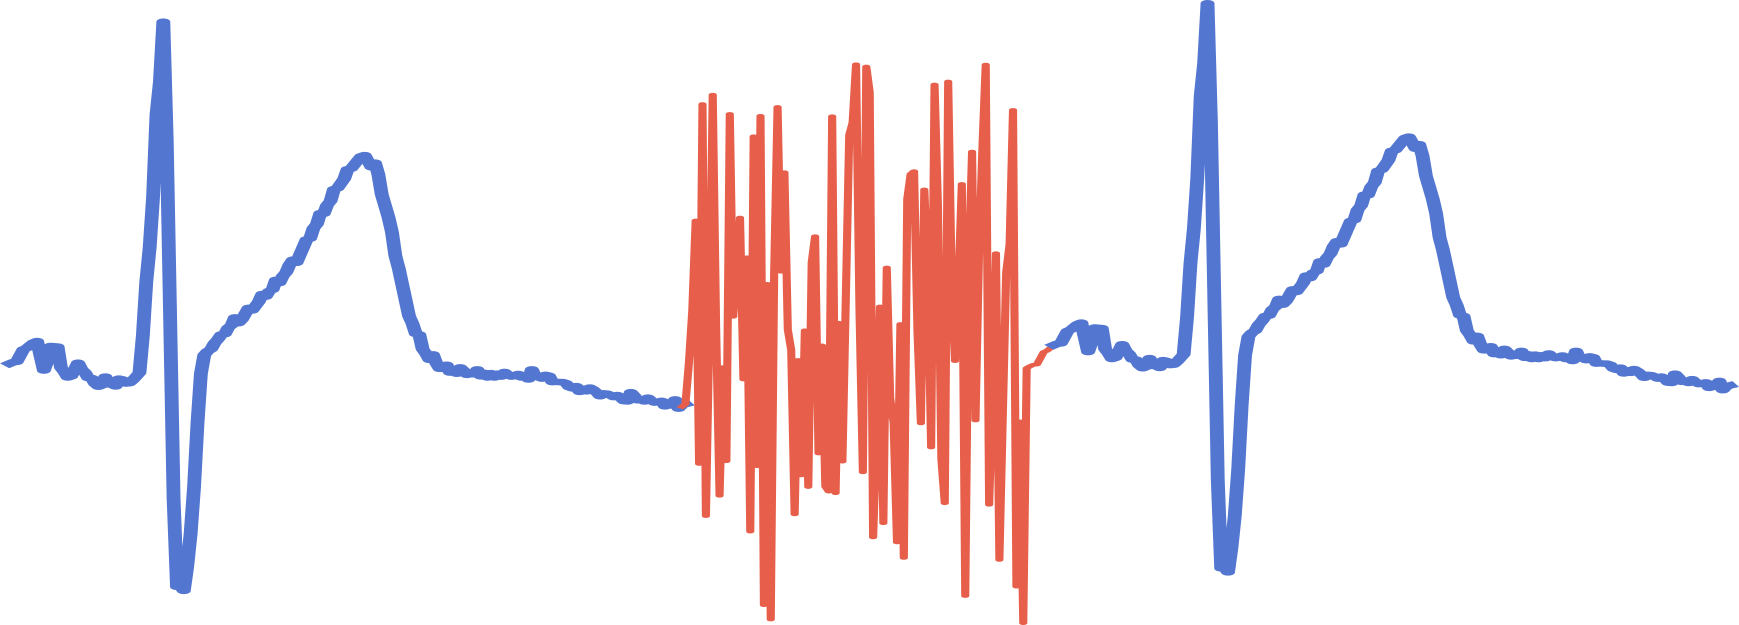
\includegraphics[height=3ex, valign=m]{ecg_noise_thumbnail.png}). When interpreting this signal, we see that it has 3 representative segments and that the first is very similar to the third one. We could then represent the signal by \textit{\textcolor{myblue}{A} \textcolor{myred}{B} \textcolor{myblue}{A}}. Some shapes may be harder to distinguish, for instance, consider an accelerometer signal of a subject while \textcolor{myblue}{walking} and shifting to \textcolor{mygreen}{jogging} regime (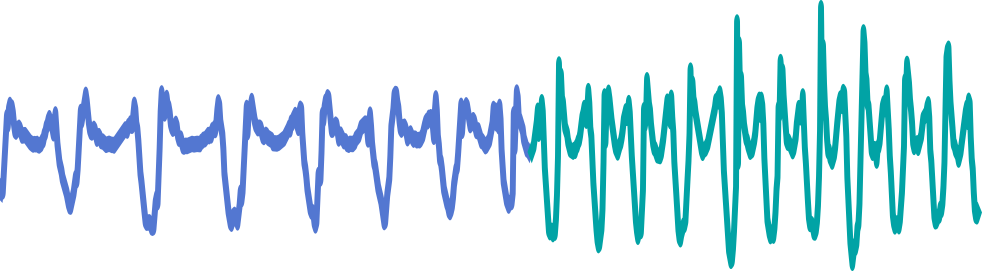
\includegraphics[height=3.5ex, valign=m]{walking_jogging.png}). Or a change in the shape of the arterial blood pressure (ABP) signal when there is a change in the subject's posture (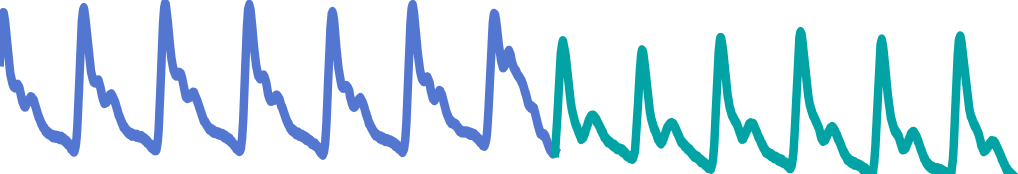
\includegraphics[height=2.5ex, valign=m]{bvpABpng.png}). In both cases, the signal has 2 structures of a similar representative periodic pattern (\textcolor{myblue}{A} \textcolor{mygreen}{B}).

This visual intuition is also very clear when a (non-)experience analyst is searching for specific shapes or patterns in time series. The reader may agree that scientists or other professionals often resort to describe the shape they are looking for. For instance, a physician may say "\textit{I am searching for the T-wave, that represents the} \texttt{large peak}" (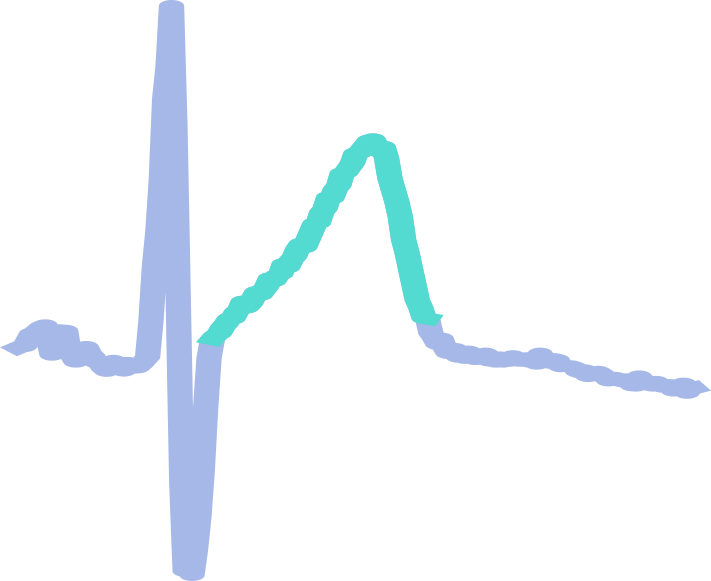
\includegraphics[height=3.5ex, valign=m]{large_peak_ecg.png}) or "\textit{I am searching for the QRS complex, that looks like a} \texttt{sharp peak followed by a sharp valley} (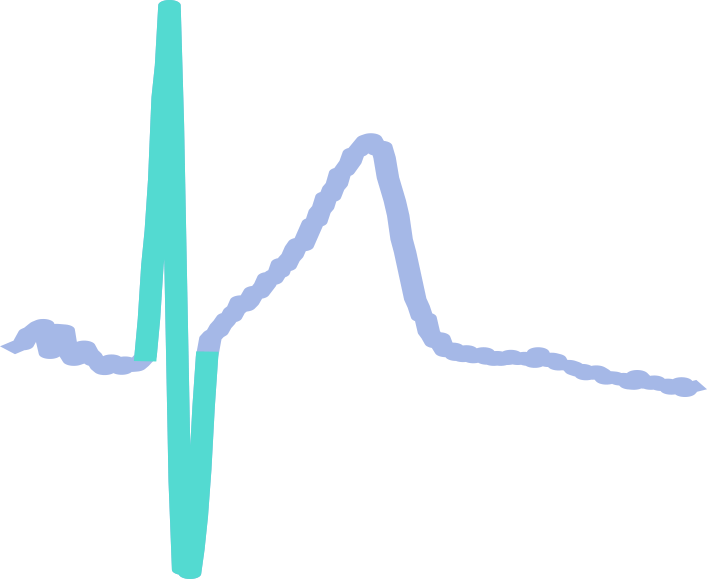
\includegraphics[height=3.5ex, valign=m]{high_peak_ecg.png})". This visual intuition also happens when analysts are trying to find differences between classes of signals. For instance, the following shapes (1) 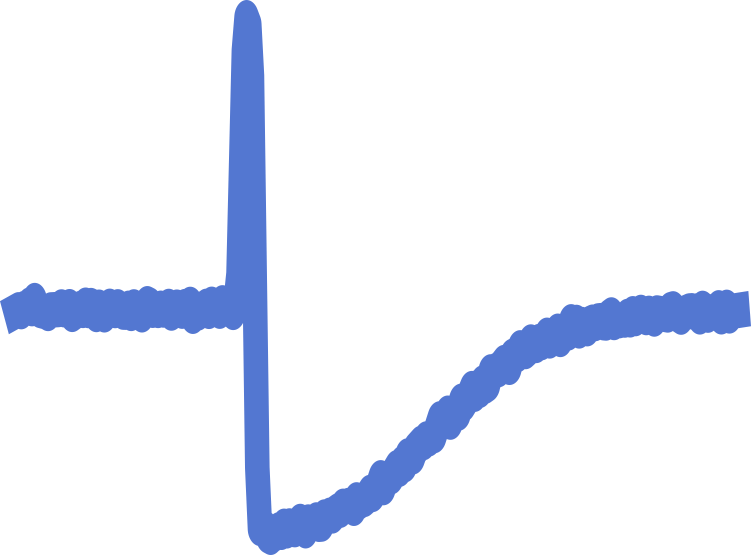
\includegraphics[height=2.5ex, width=3.5ex, valign=M]{trace1.png} and (2) 
\includegraphics[height=2.5ex, width=3.5ex, valign=M]{trace_2.png} are different because "\textit{shape 1 has a} \texttt{peak} \textit{where shape 2 doesn't}". 

Time series are carriers of information and the presence of a change in the regimes of a time series or the presence of a specific shape in a segment of a time series may be associated with a specific occurrence in the physical world and be attributed a meaning. This notion of structure and meaning is a good approximation of what represents the foundation of a language: grammar and meaning \cite{grammar}.

\textit{Grammar} is generally defined as the book of rules that constitutes the structure of a language, and is modeled by the morphology and syntax \cite{grammar}. The first is the structure of words, how these are built or morphed based on context, while the latter consists in organizing words in sequences to form larger linguistic units, such as sentences. Such as a language has morphological and syntax rules that represent its structural information, time series are also organized by a formal structure of ordered subsegments with specific morphological characteristics, organized to build larger segments.
This introduces why this thesis is designated \textit{grammar of time} and also introduces the reader further to the problematic that will be explored in this work. We will demonstrate how the developed solutions are helpful to several domains, with a special interest in showing how these can be helpful and meaningful in the context of occupational health.

\section{Context and Relevance in Occupational Health} 
\label{sub:context2}

Work-related musculoskeletal disorders (WMSDs) prevail as the most common occupational disease in the European Union. These have a global impact on the well being of individuals and their quality of life in a range of working sectors \cite{Irastorza2010}, accounting for the second largest responsibility to disability worldwilde \cite{Luttmann2003}. These are specially prevalent as upper limb or neck disorder (with 42\% of all WMSDs cases reported)~\cite{Seidel2019} in several industry sectors, such as textile and automotive, where production processes with pre-defined motions and actions have a repetitive/cyclic nature. This has a negative impact on the risk to develop musculoskeletal disorders, with tremendous consequences to both workers and companies, leading to absenteism, early retirement and loss of productivity \cite{Trabalhadores, Varandas19}. 

Several strategies have been implemented to identify, regulate and prevent occupational risk in manufacturing industries, such as (1) the inclusion of job rotation schedules, which promote a variation of the exposure throughout the working day \cite{jobrotation} and (2) screening tools, for the assessment of occupational risk exposure, e.g. OCcupational Repetitive Action (OCRA), Rapid Upper Limb Assessment (RULA) or the Ergonomic Assessment WorkSheet (EAWS) \cite{ocra, rula, eaws}. Nevertheless, these strategies are not optimal because they (1) are not automated, relying in observational methods and dedicated personal to inspect video records; (2) are not objective measures; (3) do not take into account differences among the worker's population, as anthropometric, age and experience variability; and (4) present single scores, being insufficient to explain the factors that contributed to this risk. With the advent of Industry 4.0, more companies are using modern strategies that follow digital solutions to provide direct and objective quantitative measures \cite{romero}. An example of these incentives is the usage of wearable inertial devices for motion and posture tracking of workers.

Using inertial motion units (IMUs), time series can be collected, and relevant information can be directly measured, e.g. position and velocity of each body segment, postural angles between joints and gait parameters, making these important for ergonomics studies~\cite{Caputo2019, Hang19}. There are some limitations of using IMUs, mostly related with the long term bias (sensor drifting) arising from long acquisitions and the empirical process to fine tune sensor fusion techniques. Other systems can be used for motion capture, such as camera-based methods, but these rely in fixed setup of cameras, which is unmanageable in real industrial scenarios \cite{sara}.

\textbf{SE CALHAR, INCLUIR NA MOTIVACAO QUE EM ALGUMAS EXPERIENCIAS VERIFICAMOS DIFERENCAS ENTRE GRUPO ANTROPOMETRICOS}

The usage of time series in this context can play an important role in supporting the decision of ergonomists and other professionals of the industry. In order to develop systems that can use motion and postural data for direct risk assessment and reporting, several challenges arise in the time series data mining domain. For instance, considering the periodic nature of most manufacturing tasks, risk factors are calculated by working cycle. Therefore, methods should be developed to identify working cycles with some variability in their periodicity. In addition, real occupational scenario might have interruptions or changes in the working behavior, due to abrupt production stoppage, shift breaks or even changing to another workspace that has a different motion pattern. 

Other questions also arise by ergonomists, such as "\textit{can we find a pattern that has a sharp rise in the IMU from the arm?}" or "\textit{when the worker is using a hand tool to make screwing, can we see a periodic pattern on the IMU from the hand?}, which represent specific patterns with a descriptive shape that can be seen on the signals and are specific of a task. These events can be relevant to study their precise impact on the worker's occupational exposure. Having ways to detect these patterns is of great relevance as well. In this study, we will show how the proposed solutions can have an impact in these problems, and how they contribute to provide relevant visual feedback for information retrieval from the occupational data and make the search of specific patterns more intuitive and expressive, even for non-experienced data analysts, such as ergonomists.

%This would also help counteract the lack of usability of data by moving towards a \textit{democratized} usage of time series by non-experienced scientists \cite{democratize}.

\section{Research Questions}

The previous sections introduced our main motivations related with the development of methods for information retrieval, provided context regarding the grammar of time framework and how the proposed solutions can have a significant contributions in occupational health assesment.
\par
This project addresses all the range of topics of time series, from the moment data is acquired (\textit{sensing}), processed for information retrieval (\textit{analysis}) and how it is used to act upon (\textit{decision making}). The main objectives are related with the development of methods for information retrieval (\textit{analysis}) from time series for better decision making.

\begin{enumerate}
\item \textbf{Sensing} - Explore in depth the available technology to measure motion and postural variables in occupational scenarios for risk assessment. This will take into account which variables are associated with a risk, based on ergonomic standards. These measures are reaturned as time series, which are processed in the topic \textit{analyzis};

\item \textbf{Analyzis} - In this topic, several research paths are explored. \textbf{A -} study (1) how to perform structural information retrieval in time series for segmentation based on change points and periodic points and (2) how are the segments related. For this, we applied a feature-based transformation of the time series and similarity based measures to make a meaningful visual representation, from which the segmentation points can be extracted. \textbf{B -} explore symbolic representations of time series, studying how these can be used for more expressive and intuitive pattern search with the help of regular expressions and ultimately natural language. \textbf{C -} From the textual representation of time series, study if we can make a higher leveled distance measure, following standard text mining methods. The resulting outputs of these methods can be used to get relevant information to take better decisions, namely in the occupational domain;

\item \textbf{Decision Making -} Study meaningful summarization techniques and explore several real-life examples in how the developed methods can help analysts be more aware of the data and move towards a more \textit{democratized} usage of data mining tools for information retrieval in time series. 

\end{enumerate}

With this work, we intend to contribubte to the state of the art in time series data mining with tools that provide more meaningful representations of time series, from which information can be retrieved with more meaning and at a higher level of abstraction, closer to the human intuition and visual interpretative abilities. This contributes towards more expressive methods and a democratization of these tools to accelerate the analysis process by experts in data mining and make non-experts capable of making high-level analysis.


\section{Thesis Structure}
\label{sec:structure}

This thesis provides a detailed description and explanation of the research work developed during the PhD program. It is organized in blablabla...


Figure X illustrates a guideline of the structure of this work, with a short description of each Chapter's content and description.

Chapter 1 introduced the main motivations, goals and context for the development of this thesis. Chapter 2 introduces theoretical concepts necessary to have a complete understanding of the work developed. It covers an introduction to motion and postural sensors used in occupational settings, time series, standard methods for its representation and analysis and text mining concepts. Chapter 3 presents the most recent works related with what we developed, namely in the topics of segmentation, summarization, pattern/event search and dictionnary based classification. On Chapter 4 we start describing the data we used, explaining its source for both acquired data and publicly available, for what it was used and how. It includes a detailed description of the protocol used to acquired workers' motion data in real industrial scenarios. The algorithm developed for time series structural information retrieval is explained in Chapter 5, while Chapter 6 covers the symbolic representation of time series. In this chapter is explained the exploratory path to use this novel representation in query search and classification tasks. Chapter 7 shows the application of the previous methods to an exaustive set of examples, namely from the occupational scenario, and major results are presented. In addition, this chapter also provide a general discussion about the usage of these methods for decision making. Finally, Chapter 8 gives an overall remark over the outcomes of this thesis and a reflection over the contributions that the developed methods have in making time series preparation and data mining more expressive, quicker and more practicle for an ever increasing number of data available. Each chapter will have a short introduction to situate and contextualize the reader.
